\newpage
\section{Описание протокола}

На рисунке \ref{img:key_hierarchy} представлена иерархия ключей в EAP-PSK.

\begin{figure}[h!]
\center{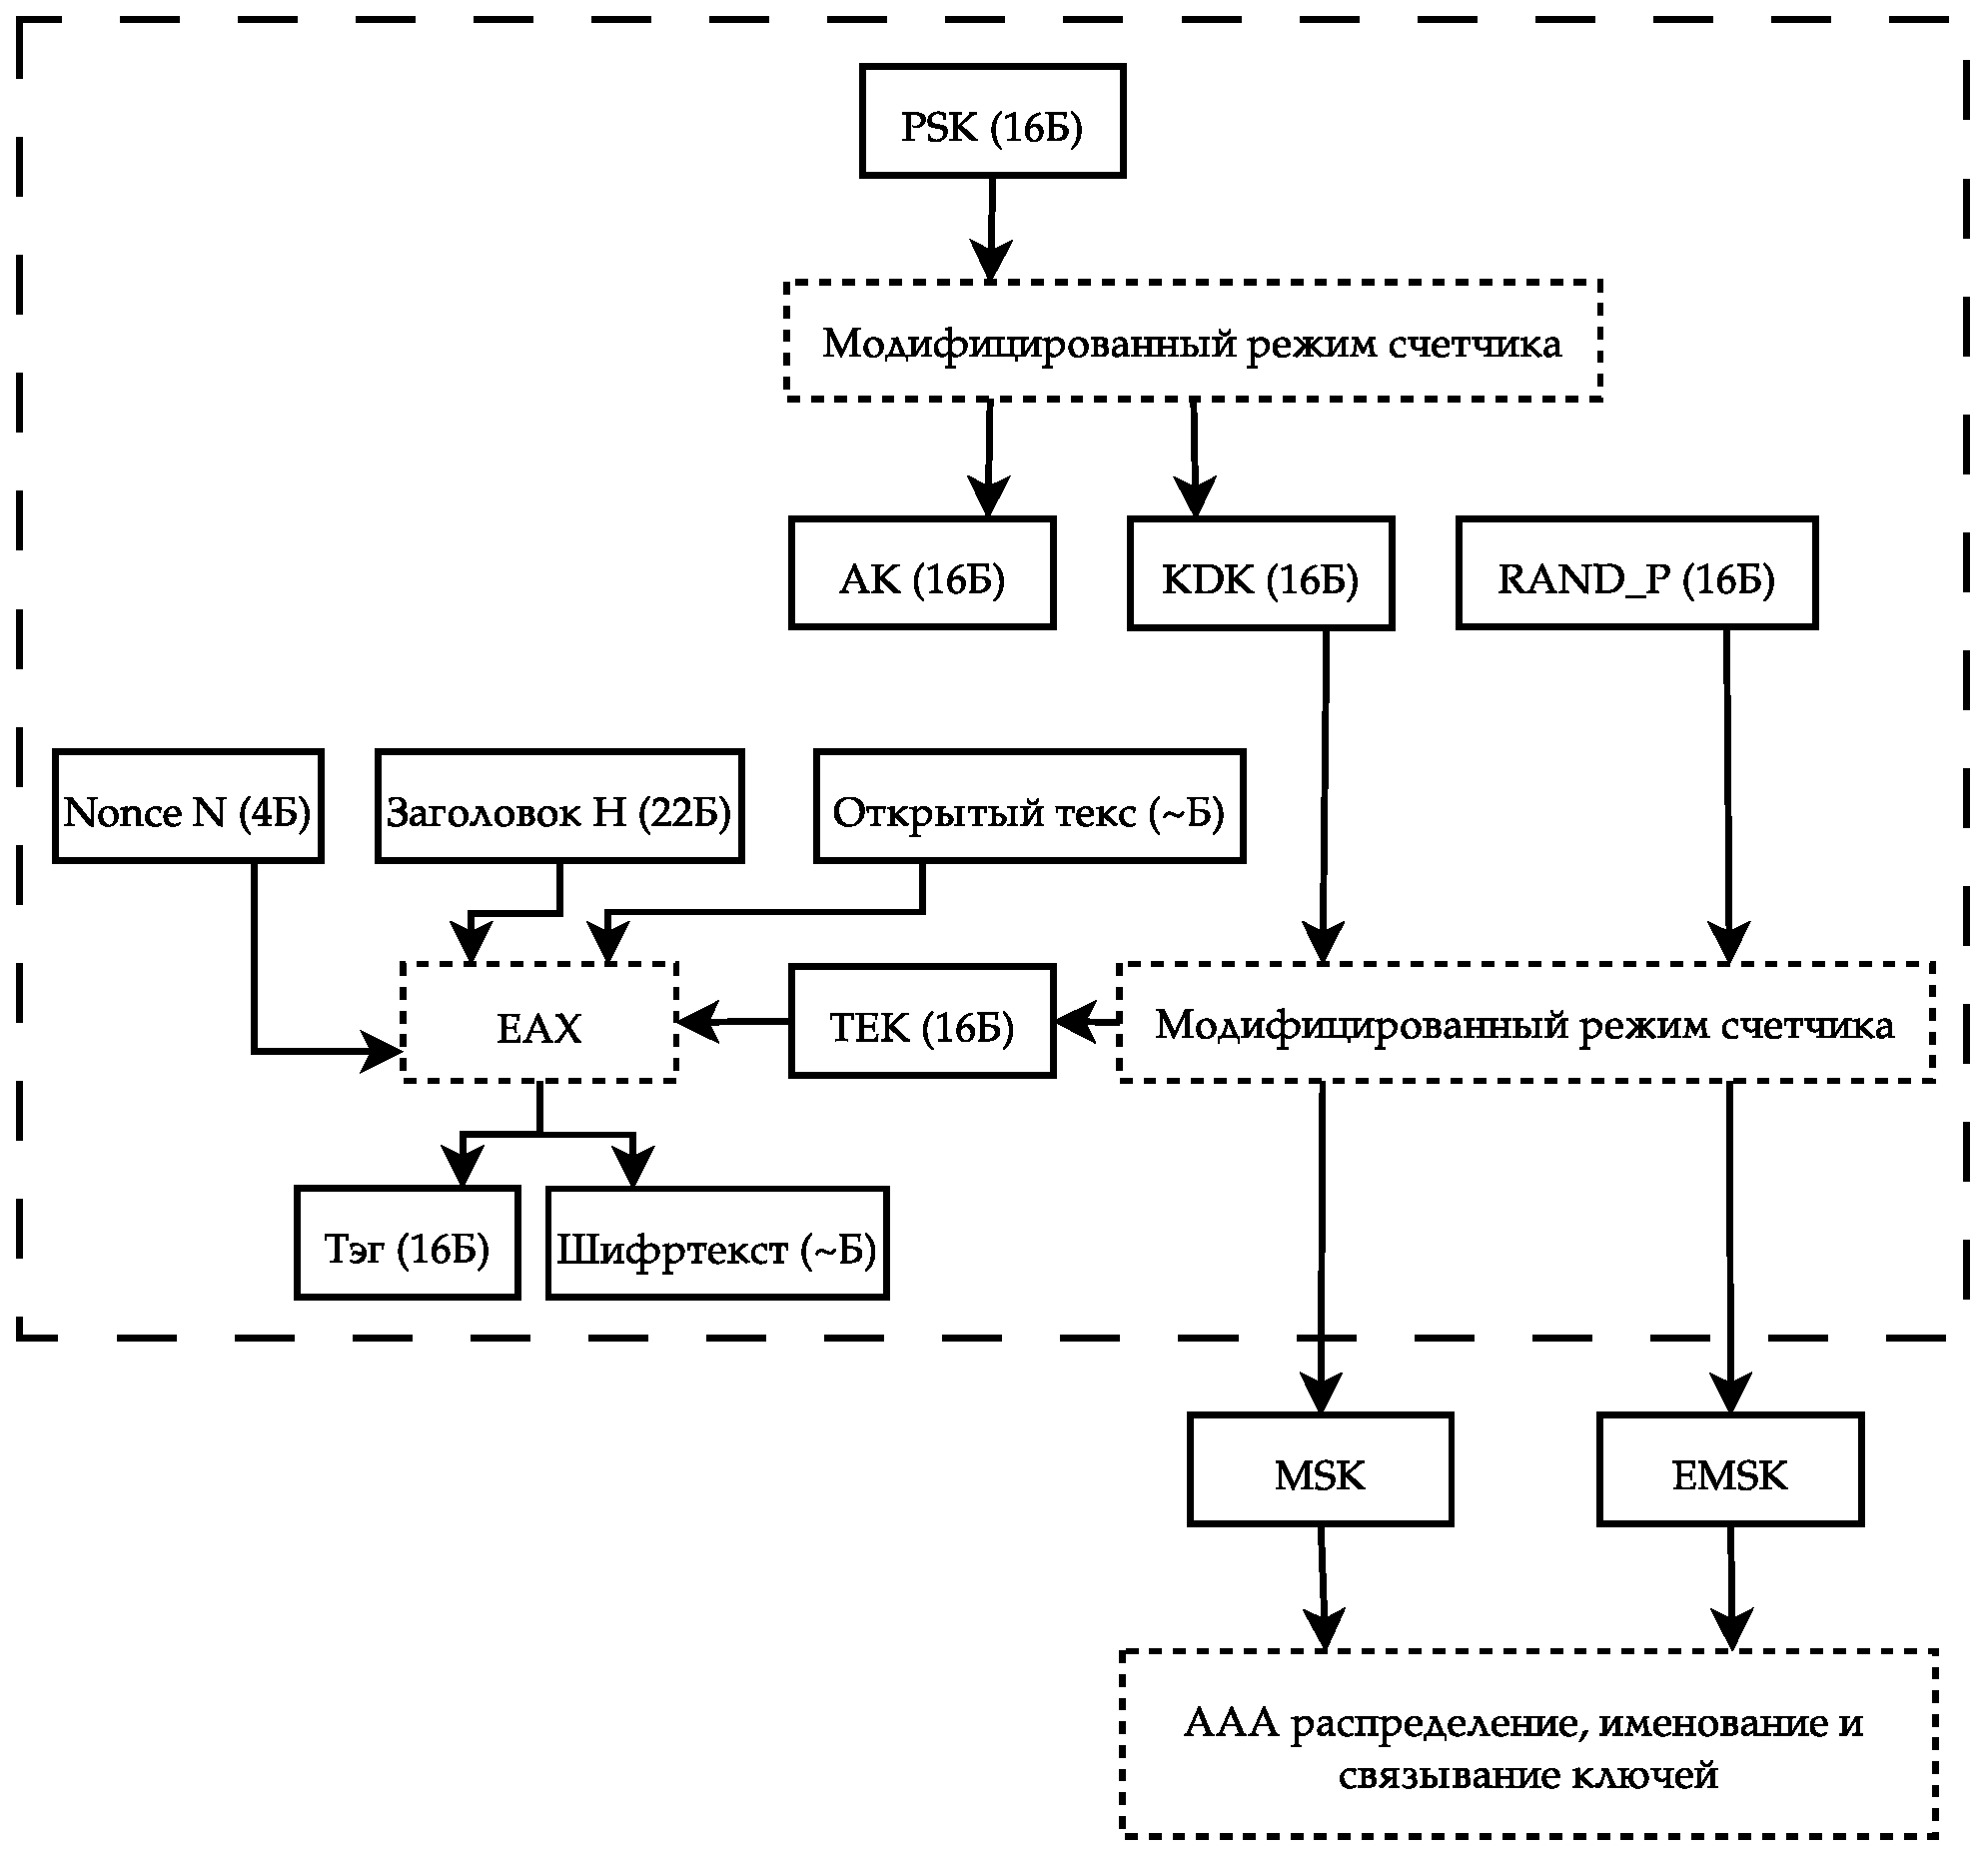
\includegraphics[width=0.9\linewidth]{./pictures/key_hierarchy}}
\caption{Описание иерархии ключей в EAP-PSK}
\label{img:key_hierarchy}
\end{figure}

\subsection{Иерархия ключей EAP-PSK}

В данном разделе описывается иерархия ключей, использующаяся в EAP-PSK. Эта иерархия базирутся на иерархии, оаисанной в документе ``Extensible Authentication Protocol (EAP) Key Management Framework''

\subsubsection{PSK}

PSK распределяется между Пиром и сервером.


